\documentclass[9pt]{beamer}

\usepackage[utf8x]{inputenc}
\usepackage[english]{babel}
\usepackage{amsmath, amsfonts, amssymb}
\usepackage{color}
\usepackage{xcolor}
\usepackage{tikz}
\usetikzlibrary{positioning,shapes,shadows,arrows,snakes}
\usepackage{listliketab}
\usepackage{shuffle}
\usepackage{xargs}
\usepackage{multirow}
\usepackage{pgfplots}
\usepackage{csquotes}
\usepackage{verbatim}

\definecolor{BlueGreen}{cmyk}{0.85,0,0.33,0}
\definecolor{RawSienna}{cmyk}{0,0.72,1,0.45}
\definecolor{gold}{rgb}{1.,0.84,0.}
\definecolor{dgreen}{rgb}{0.,0.6,0.}

\definecolor{Noir}{RGB}{0,0,0}
\definecolor{Rouge}{RGB}{205,35,38}
\definecolor{Bleu}{RGB}{2,60,195}
\definecolor{Bleu1}{RGB}{121,176,197}
\definecolor{Vert}{RGB}{23,103,1}
\definecolor{VertOlive}{RGB}{112,141,35}
\definecolor{Orange}{RGB}{255,113,15}
\definecolor{RoseBonbon}{RGB}{249,66,158}
\definecolor{Marron}{RGB}{193,88,50}

\definecolor{mygreen}{RGB}{23,103,1}

\newcommand{\red}[1]{\textcolor{red}{#1}}
\newcommand{\blue}[1]{\textcolor{blue}{#1}}
\newcommand{\green}[1]{\textcolor{mygreen}{#1}}
\newcommand{\bluealert}[2]{\textcolor<#1>{blue}{#2}}

\tikzstyle{alert} = [color=red, line width = 1.5]
\tikzstyle{bluealert} = [color=blue, line width =1.5]
\tikzstyle{big} = [line width = 1.5]
\tikzstyle{Point} = [fill, radius=0.08]
\tikzstyle{RedPoint} = [fill, radius=0.09, color = red]


\tikzstyle{Red} = [color = red]
\tikzstyle{Blue} = [color = blue]
\tikzstyle{Green} = [color = Vert]
\tikzstyle{Gray} = [color = gray]

\definecolor{violet}{rgb}{.5,.1,.9}


\usetheme{Boadilla}
\title{Machine learning basics}
\author[G. Châtel]{Grégory Châtel\\\vspace{0.3cm}Disaitek\\Intel Software Innovator\\\vspace{0.3cm}@rodgzilla\\github.com/rodgzilla\\\vspace{.5cm}\includegraphics[width = 2.5cm]{images/logo_disaitek.png} \vspace{-1cm}
}
\date{2019/02/12}

\begin{document}

%%%%%%%%%%%%%%%%%%%%%%%%%%%%%%%%%%%%%%%%%%%%%%%%%%%%%%%%%%%%%%%%%%%%%%
\begin{frame}

  \maketitle

\end{frame}
%%%%%%%%%%%%%%%%%%%%%%%%%%%%%%%%%%%%%%%%%%%%%%%%%%%%%%%%%%%%%%%%%%%%%%

%%%%%%%%%%%%%%%%%%%%%%%%%%%%%%%%%%%%%%%%%%%%%%%%%%%%%%%%%%%%%%%%%%%%%%
\begin{frame}

  \frametitle{Machine learning}

  Machine learning (ML) is a subfield of artificial intelligence.

  \bigskip

  \begin{description}
    \item[Intuitively] We want to \emph{learn from} and \emph{make predictions
    on} data.

      \medskip

    \item[Technically] We want to update the parameters of a model to
      make it describe our training data as well as possible (``well''
      being defined by a \emph{loss function}).
  \end{description}

\end{frame}
%%%%%%%%%%%%%%%%%%%%%%%%%%%%%%%%%%%%%%%%%%%%%%%%%%%%%%%%%%%%%%%%%%%%%%

%%%%%%%%%%%%%%%%%%%%%%%%%%%%%%%%%%%%%%%%%%%%%%%%%%%%%%%%%%%%%%%%%%%%%%
\begin{frame}
  \frametitle{Model example}

  \framesubtitle{Linear regression}

  \begin{center}
    \scalebox{1.3}{
      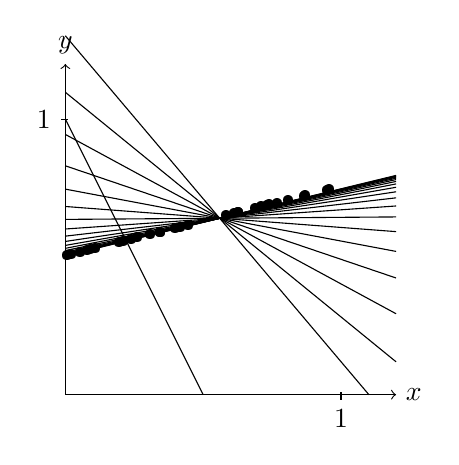
\begin{tikzpicture}[xscale = 3.5, yscale=3.5]
  \foreach \Point in { (0.418313, 0.604578), (0.196620, 0.549155),
    (0.734198, 0.683549), (0.767944, 0.691986), (0.212015, 0.553004),
    (0.866296, 0.716574), (0.741085, 0.685271), (0.091187, 0.522797),
    (0.957083, 0.739271), (0.400345, 0.600086), (0.110229, 0.527557),
    (0.628896, 0.657224), (0.079816, 0.519954), (0.585337, 0.646334),
    (0.240140, 0.560035), (0.712331, 0.678083), (0.810917, 0.702729),
    (0.262672, 0.565668), (0.690066, 0.672516), (0.871858, 0.717964),
    (0.444774, 0.611194), (0.021740, 0.505435), (0.308306, 0.577077),
    (0.055931, 0.513983), (0.343537, 0.585884), (0.007552, 0.501888),
    (0.614842, 0.653711), (0.343214, 0.585804), (0.627016, 0.656754),
    (0.951821, 0.737955) }{ 
    \node at \Point {
      \textbullet
    }; 
  }

  \draw[->] (0, 0) -- (1.2, 0) node[right] {$x$};
  \draw[->] (0, 0) -- (0, 1.2) node[above] {$y$};
  \draw (1, 0.25pt) -- (1, -0.5pt) node[anchor = north]{1};
  \draw (0.25pt, 1) -- (-0.5pt, 1) node[anchor = east]{1};
  \uncover<1>{\draw (0.000000, 1.000000) -- (0.500000, 0.000000);}
  \uncover<2>{\draw (0.000000, 1.302205) -- (1.101420, 0.000000);}
  \uncover<3>{\draw (0.000000, 1.097310) -- (1.200000, 0.119256);}
  \uncover<4>{\draw (0.000000, 0.944298) -- (1.200000, 0.293644);}
  \uncover<5>{\draw (0.000000, 0.830482) -- (1.200000, 0.423357);}
  \uncover<6>{\draw (0.000000, 0.745822) -- (1.200000, 0.519842);}
  \uncover<7>{\draw (0.000000, 0.682850) -- (1.200000, 0.591610);}
  \uncover<8>{\draw (0.000000, 0.636009) -- (1.200000, 0.644993);}
  \uncover<9>{\draw (0.000000, 0.601168) -- (1.200000, 0.684702);}
  \uncover<10>{\draw (0.000000, 0.575251) -- (1.200000, 0.714238);}
  \uncover<11>{\draw (0.000000, 0.555974) -- (1.200000, 0.736207);}
  \uncover<12>{\draw (0.000000, 0.541635) -- (1.200000, 0.752549);}
  \uncover<13>{\draw (0.000000, 0.530970) -- (1.200000, 0.764705);}
  \uncover<14>{\draw (0.000000, 0.523036) -- (1.200000, 0.773746);}
  \uncover<15>{\draw (0.000000, 0.517135) -- (1.200000, 0.780472);}
  \uncover<16>{\draw (0.000000, 0.512745) -- (1.200000, 0.785474);}
  \uncover<17>{\draw (0.000000, 0.509480) -- (1.200000, 0.789195);}
  \uncover<18>{\draw (0.000000, 0.507052) -- (1.200000, 0.791963);}
  \uncover<19>{\draw (0.000000, 0.505245) -- (1.200000, 0.794022);}
  \uncover<20>{\draw (0.000000, 0.503902) -- (1.200000, 0.795553);}
\end{tikzpicture}

    }
  \end{center}

\end{frame}
%%%%%%%%%%%%%%%%%%%%%%%%%%%%%%%%%%%%%%%%%%%%%%%%%%%%%%%%%%%%%%%%%%%%%%

%%%%%%%%%%%%%%%%%%%%%%%%%%%%%%%%%%%%%%%%%%%%%%%%%%%%%%%%%%%%%%%%%%%%%%
\begin{frame}
  \frametitle{Model example}

  \framesubtitle{Decision tree}

  \begin{center}
    \includegraphics[width = 9cm]{images/decision_tree.png}
  \end{center}

\end{frame}
%%%%%%%%%%%%%%%%%%%%%%%%%%%%%%%%%%%%%%%%%%%%%%%%%%%%%%%%%%%%%%%%%%%%%%

%%%%%%%%%%%%%%%%%%%%%%%%%%%%%%%%%%%%%%%%%%%%%%%%%%%%%%%%%%%%%%%%%%%%%%
\begin{frame}
  \frametitle{Model example}

  \framesubtitle{Neural network (deep learning)}

  \begin{center}
    \scalebox{0.7}{
      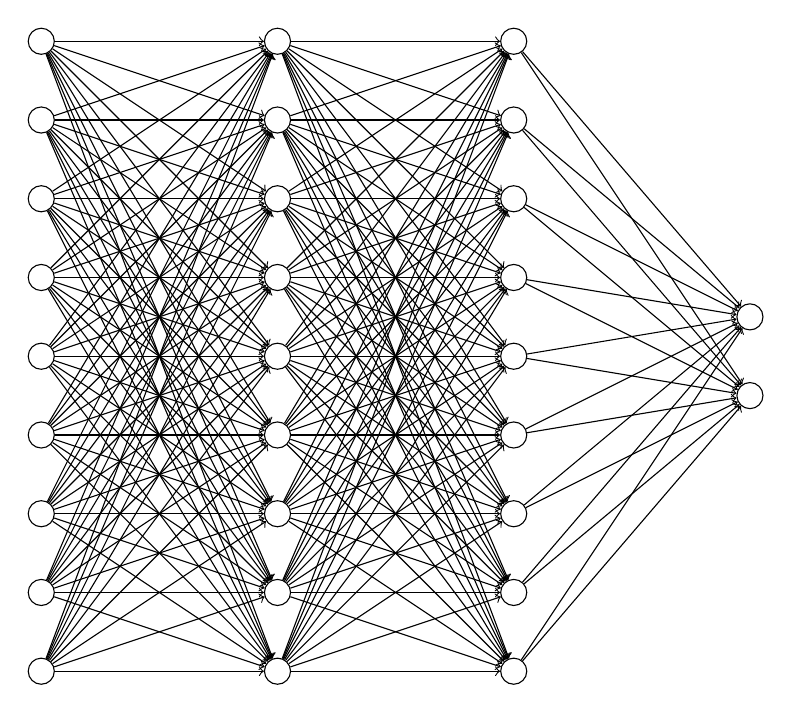
\begin{tikzpicture}[xscale = 3]
  \node[draw, circle] (N11) at (0, 0){
  };

  \node[draw, circle] (N21) at (0, -1){
  };

  \node[draw, circle] (N31) at (0, -2){
  };

  \node[draw, circle] (N41) at (0, -3){
  };

  \node[draw, circle] (N51) at (0, -4){
  };

  \node[draw, circle] (N61) at (0, -5){
  };

  \node[draw, circle] (N71) at (0, -6){
  };

  \node[draw, circle] (N81) at (0, -7){
  };

  \node[draw, circle] (N91) at (0, -8){
  };

  \node[draw, circle] (N12) at (1, 0){
  };

  \node[draw, circle] (N22) at (1, -1){
  };

  \node[draw, circle] (N32) at (1, -2){
  };

  \node[draw, circle] (N42) at (1, -3){
  };

  \node[draw, circle] (N52) at (1, -4){
  };

  \node[draw, circle] (N62) at (1, -5){
  };

  \node[draw, circle] (N72) at (1, -6){
  };

  \node[draw, circle] (N82) at (1, -7){
  };

  \node[draw, circle] (N92) at (1, -8){
  };

  \node[draw, circle] (N13) at (2, 0){
  };

  \node[draw, circle] (N23) at (2, -1){
  };

  \node[draw, circle] (N33) at (2, -2){
  };

  \node[draw, circle] (N43) at (2, -3){
  };

  \node[draw, circle] (N53) at (2, -4){
  };

  \node[draw, circle] (N63) at (2, -5){
  };

  \node[draw, circle] (N73) at (2, -6){
  };

  \node[draw, circle] (N83) at (2, -7){
  };

  \node[draw, circle] (N93) at (2, -8){
  };

  \node[draw, circle] (N14) at (3, -3.5){
  };

  \node[draw, circle] (N24) at (3, -4.5){
  };

  \draw[->] (N11) -- (N12);
  \draw[->] (N11) -- (N22);
  \draw[->] (N11) -- (N32);
  \draw[->] (N11) -- (N42);
  \draw[->] (N11) -- (N52);
  \draw[->] (N11) -- (N62);
  \draw[->] (N11) -- (N72);
  \draw[->] (N11) -- (N82);
  \draw[->] (N11) -- (N92);
  \draw[->] (N21) -- (N12);
  \draw[->] (N21) -- (N22);
  \draw[->] (N21) -- (N32);
  \draw[->] (N21) -- (N42);
  \draw[->] (N21) -- (N52);
  \draw[->] (N21) -- (N62);
  \draw[->] (N21) -- (N72);
  \draw[->] (N21) -- (N82);
  \draw[->] (N21) -- (N92);
  \draw[->] (N31) -- (N12);
  \draw[->] (N31) -- (N22);
  \draw[->] (N31) -- (N32);
  \draw[->] (N31) -- (N42);
  \draw[->] (N31) -- (N52);
  \draw[->] (N31) -- (N62);
  \draw[->] (N31) -- (N72);
  \draw[->] (N31) -- (N82);
  \draw[->] (N31) -- (N92);
  \draw[->] (N41) -- (N12);
  \draw[->] (N41) -- (N22);
  \draw[->] (N41) -- (N32);
  \draw[->] (N41) -- (N42);
  \draw[->] (N41) -- (N52);
  \draw[->] (N41) -- (N62);
  \draw[->] (N41) -- (N72);
  \draw[->] (N41) -- (N82);
  \draw[->] (N41) -- (N92);
  \draw[->] (N51) -- (N12);
  \draw[->] (N51) -- (N22);
  \draw[->] (N51) -- (N32);
  \draw[->] (N51) -- (N42);
  \draw[->] (N51) -- (N52);
  \draw[->] (N51) -- (N62);
  \draw[->] (N51) -- (N72);
  \draw[->] (N51) -- (N82);
  \draw[->] (N51) -- (N92);
  \draw[->] (N61) -- (N12);
  \draw[->] (N61) -- (N22);
  \draw[->] (N61) -- (N32);
  \draw[->] (N61) -- (N42);
  \draw[->] (N61) -- (N52);
  \draw[->] (N61) -- (N62);
  \draw[->] (N61) -- (N72);
  \draw[->] (N61) -- (N82);
  \draw[->] (N61) -- (N92);
  \draw[->] (N71) -- (N12);
  \draw[->] (N71) -- (N22);
  \draw[->] (N71) -- (N32);
  \draw[->] (N71) -- (N42);
  \draw[->] (N71) -- (N52);
  \draw[->] (N71) -- (N62);
  \draw[->] (N71) -- (N72);
  \draw[->] (N71) -- (N82);
  \draw[->] (N71) -- (N92);
  \draw[->] (N81) -- (N12);
  \draw[->] (N81) -- (N22);
  \draw[->] (N81) -- (N32);
  \draw[->] (N81) -- (N42);
  \draw[->] (N81) -- (N52);
  \draw[->] (N81) -- (N62);
  \draw[->] (N81) -- (N72);
  \draw[->] (N81) -- (N82);
  \draw[->] (N81) -- (N92);
  \draw[->] (N91) -- (N12);
  \draw[->] (N91) -- (N22);
  \draw[->] (N91) -- (N32);
  \draw[->] (N91) -- (N42);
  \draw[->] (N91) -- (N52);
  \draw[->] (N91) -- (N62);
  \draw[->] (N91) -- (N72);
  \draw[->] (N91) -- (N82);
  \draw[->] (N91) -- (N92);
  \draw[->] (N12) -- (N13);
  \draw[->] (N12) -- (N23);
  \draw[->] (N12) -- (N33);
  \draw[->] (N12) -- (N43);
  \draw[->] (N12) -- (N53);
  \draw[->] (N12) -- (N63);
  \draw[->] (N12) -- (N73);
  \draw[->] (N12) -- (N83);
  \draw[->] (N12) -- (N93);
  \draw[->] (N22) -- (N13);
  \draw[->] (N22) -- (N23);
  \draw[->] (N22) -- (N33);
  \draw[->] (N22) -- (N43);
  \draw[->] (N22) -- (N53);
  \draw[->] (N22) -- (N63);
  \draw[->] (N22) -- (N73);
  \draw[->] (N22) -- (N83);
  \draw[->] (N22) -- (N93);
  \draw[->] (N32) -- (N13);
  \draw[->] (N32) -- (N23);
  \draw[->] (N32) -- (N33);
  \draw[->] (N32) -- (N43);
  \draw[->] (N32) -- (N53);
  \draw[->] (N32) -- (N63);
  \draw[->] (N32) -- (N73);
  \draw[->] (N32) -- (N83);
  \draw[->] (N32) -- (N93);
  \draw[->] (N42) -- (N13);
  \draw[->] (N42) -- (N23);
  \draw[->] (N42) -- (N33);
  \draw[->] (N42) -- (N43);
  \draw[->] (N42) -- (N53);
  \draw[->] (N42) -- (N63);
  \draw[->] (N42) -- (N73);
  \draw[->] (N42) -- (N83);
  \draw[->] (N42) -- (N93);
  \draw[->] (N52) -- (N13);
  \draw[->] (N52) -- (N23);
  \draw[->] (N52) -- (N33);
  \draw[->] (N52) -- (N43);
  \draw[->] (N52) -- (N53);
  \draw[->] (N52) -- (N63);
  \draw[->] (N52) -- (N73);
  \draw[->] (N52) -- (N83);
  \draw[->] (N52) -- (N93);
  \draw[->] (N62) -- (N13);
  \draw[->] (N62) -- (N23);
  \draw[->] (N62) -- (N33);
  \draw[->] (N62) -- (N43);
  \draw[->] (N62) -- (N53);
  \draw[->] (N62) -- (N63);
  \draw[->] (N62) -- (N73);
  \draw[->] (N62) -- (N83);
  \draw[->] (N62) -- (N93);
  \draw[->] (N72) -- (N13);
  \draw[->] (N72) -- (N23);
  \draw[->] (N72) -- (N33);
  \draw[->] (N72) -- (N43);
  \draw[->] (N72) -- (N53);
  \draw[->] (N72) -- (N63);
  \draw[->] (N72) -- (N73);
  \draw[->] (N72) -- (N83);
  \draw[->] (N72) -- (N93);
  \draw[->] (N82) -- (N13);
  \draw[->] (N82) -- (N23);
  \draw[->] (N82) -- (N33);
  \draw[->] (N82) -- (N43);
  \draw[->] (N82) -- (N53);
  \draw[->] (N82) -- (N63);
  \draw[->] (N82) -- (N73);
  \draw[->] (N82) -- (N83);
  \draw[->] (N82) -- (N93);
  \draw[->] (N92) -- (N13);
  \draw[->] (N92) -- (N23);
  \draw[->] (N92) -- (N33);
  \draw[->] (N92) -- (N43);
  \draw[->] (N92) -- (N53);
  \draw[->] (N92) -- (N63);
  \draw[->] (N92) -- (N73);
  \draw[->] (N92) -- (N83);
  \draw[->] (N92) -- (N93);
  \draw[->] (N13) -- (N14);
  \draw[->] (N13) -- (N24);
  \draw[->] (N23) -- (N14);
  \draw[->] (N23) -- (N24);
  \draw[->] (N33) -- (N14);
  \draw[->] (N33) -- (N24);
  \draw[->] (N43) -- (N14);
  \draw[->] (N43) -- (N24);
  \draw[->] (N53) -- (N14);
  \draw[->] (N53) -- (N24);
  \draw[->] (N63) -- (N14);
  \draw[->] (N63) -- (N24);
  \draw[->] (N73) -- (N14);
  \draw[->] (N73) -- (N24);
  \draw[->] (N83) -- (N14);
  \draw[->] (N83) -- (N24);
  \draw[->] (N93) -- (N14);
  \draw[->] (N93) -- (N24);

\end{tikzpicture}

    }
  \end{center}
\end{frame}
%%%%%%%%%%%%%%%%%%%%%%%%%%%%%%%%%%%%%%%%%%%%%%%%%%%%%%%%%%%%%%%%%%%%%%

%%%%%%%%%%%%%%%%%%%%%%%%%%%%%%%%%%%%%%%%%%%%%%%%%%%%%%%%%%%%%%%%%%%%%%
\begin{frame}
  \frametitle{Deep learning architecture}

  \framesubtitle{Image recognition (VGG 16)}

  \begin{center}
    \includegraphics[width = 9cm]{images/vgg16_architecture.png}
  \end{center}

\end{frame}
%%%%%%%%%%%%%%%%%%%%%%%%%%%%%%%%%%%%%%%%%%%%%%%%%%%%%%%%%%%%%%%%%%%%%%

%%%%%%%%%%%%%%%%%%%%%%%%%%%%%%%%%%%%%%%%%%%%%%%%%%%%%%%%%%%%%%%%%%%%%%
\begin{frame}
  \frametitle{Deep learning architecture}

  \framesubtitle{Hierarchized pattern recognition}

  \begin{center}
    \begin{tikzpicture}[xscale = 5.5, yscale = 2.5]
      \onslide<1>{
        \node (L1) at (0, 0) {
          \includegraphics[width = 5cm]{images/cnn_vizu_l1.jpg}
        };

        \node (T1) at (-1, 0.5) {
          Layer 1
        };
      }
      \onslide<2>{
        \node (L2) at (0, 0) {
          \includegraphics[width = 5cm]{images/cnn_vizu_l2.jpg}
        };

        \node (T2) at (-1, 0.5) {
          Layer 2
        };
            }
      \onslide<3>{
        \node (L3) at (0, 0) {
          \includegraphics[width = 5cm]{images/cnn_vizu_l3.jpg}
        };

        \node (T3) at (-1, 0.5) {
          Layer 3
        };
            }
      \onslide<4>{
        \node (L4) at (0, 0) {
          \includegraphics[width = 5cm]{images/cnn_vizu_l4.jpg}
        };
        \node (T4) at (-1, 0.5) {
          Layer 4
        };
            }
      \onslide<5>{
        \node (L5) at (0, 0) {
          \includegraphics[width = 5cm]{images/cnn_vizu_l5.jpg}
        };

        \node (T5) at (-1, 0.5) {
          Layer 5
        };
      }

      \node (VGG) at (-1, -0.5) {
        \includegraphics[width = 6cm]{images/vgg16_architecture.png}
      };
    \end{tikzpicture}
  \end{center}

\end{frame}
%%%%%%%%%%%%%%%%%%%%%%%%%%%%%%%%%%%%%%%%%%%%%%%%%%%%%%%%%%%%%%%%%%%%%%

%%%%%%%%%%%%%%%%%%%%%%%%%%%%%%%%%%%%%%%%%%%%%%%%%%%%%%%%%%%%%%%%%%%%%%
\begin{frame}

  \frametitle{Application examples}

  \framesubtitle{Supervised learning}

  \begin{itemize}
    \item Supervised tasks
      \begin{itemize}
      \item Regression

        \begin{center}
          \begin{tabular}{cc}
            \textcolor{blue}{Recommender system} & (user, book) $\to$ rating \\[0.2cm]
            \textcolor{blue}{House price} & (surface, nb rooms, city) $\to$ price \\[0.2cm]
        \end{tabular}
        \end{center}

      \item Classification

        \begin{center}
          \begin{tabular}{cc}
            \textcolor{blue}{Image classification} & pixel values $\to$ cat or dog \\[0.2cm]
            \textcolor{blue}{Text classification} & list of words $\to$ spam or valid email
          \end{tabular}
        \end{center}
      \end{itemize}
    \item Unsupervised tasks

      \begin{itemize}
        \item Clustering
          \begin{center}
            \textcolor{blue}{Group clients by interests} \\[.5cm]
          \end{center}
        \item Anomaly detection
          \begin{center}
            \textcolor{blue}{Credit card fraud detection}
          \end{center}
      \end{itemize}
  \end{itemize}

\end{frame}
%%%%%%%%%%%%%%%%%%%%%%%%%%%%%%%%%%%%%%%%%%%%%%%%%%%%%%%%%%%%%%%%%%%%%%

%%%%%%%%%%%%%%%%%%%%%%%%%%%%%%%%%%%%%%%%%%%%%%%%%%%%%%%%%%%%%%%%%%%%%%
\begin{frame}
  \frametitle{Deep Natural Language Processing (NLP)}

  \framesubtitle{Main ideas}

  \begin{itemize}
    \item Learning the \textcolor{blue}{semantic meaning} of words,
      \pause
      \bigskip
    \item Understanding the \textcolor{blue}{information hierarchy} related to
      the task at hand,
      \bigskip
      \pause
    \item Ability to make use of \textcolor{blue}{huge amounts of data}.
  \end{itemize}
\end{frame}
%%%%%%%%%%%%%%%%%%%%%%%%%%%%%%%%%%%%%%%%%%%%%%%%%%%%%%%%%%%%%%%%%%%%%%

%%%%%%%%%%%%%%%%%%%%%%%%%%%%%%%%%%%%%%%%%%%%%%%%%%%%%%%%%%%%%%%%%%%%%%
\begin{frame}
  \frametitle{Word embeddings}

  \framesubtitle{Semantic vectors}

  We associate to each word of the vocabulary a vector which
  represents its \textcolor{blue}{meaning}.

  \begin{center}
    \begin{description}
      \item[Oven] $[-0.2, 0.6]$
      \item[Microwave] $[-0.05, 0.57]$
      \item[Garden] $[0.22, -0.5]$
      \item \dots
    \end{description}
  \end{center}

  \vspace{-.9cm}

  \begin{center}
    \includegraphics[width = 8.5cm]{images/word_embeddings_5.png}
  \end{center}

  \vspace{-0.5cm}

  In real applications word embedding have 100 to 300 values,
  encoding all kind of characteristics about words.
\end{frame}
%%%%%%%%%%%%%%%%%%%%%%%%%%%%%%%%%%%%%%%%%%%%%%%%%%%%%%%%%%%%%%%%%%%%%%

%%%%%%%%%%%%%%%%%%%%%%%%%%%%%%%%%%%%%%%%%%%%%%%%%%%%%%%%%%%%%%%%%%%%%%
\begin{frame}
  \frametitle{Word embeddings}

  \framesubtitle{Links between concepts}

  When word embeddings are created using a large enough dataset, a lot
  of information is encoded in \textcolor{blue}{differences} between
  vectors.

  \begin{center}
    \includegraphics[width = 8cm]{images/word_embeddings_3.png}
  \end{center}
\end{frame}
%%%%%%%%%%%%%%%%%%%%%%%%%%%%%%%%%%%%%%%%%%%%%%%%%%%%%%%%%%%%%%%%%%%%%%

%%%%%%%%%%%%%%%%%%%%%%%%%%%%%%%%%%%%%%%%%%%%%%%%%%%%%%%%%%%%%%%%%%%%%%
\begin{frame}
  \frametitle{Word embeddings}

  \framesubtitle{Vector geometry}

  \begin{center}
    \includegraphics[width = 5cm]{images/word_embeddings_2.png}
  \end{center}
  \[
  king - man + woman = queen
  \]
  \begin{center}
    \includegraphics[width = 3.5cm]{images/king_queen.png}
  \end{center}
\end{frame}
%%%%%%%%%%%%%%%%%%%%%%%%%%%%%%%%%%%%%%%%%%%%%%%%%%%%%%%%%%%%%%%%%%%%%%

%%%%%%%%%%%%%%%%%%%%%%%%%%%%%%%%%%%%%%%%%%%%%%%%%%%%%%%%%%%%%%%%%%%%%%
\begin{frame}
  \frametitle{Word embeddings}

  \framesubtitle{Bias in representations}

  \begin{center}
    \includegraphics[width = 10cm]{images/nurse.png} \\[.5cm]
    \includegraphics[width = 10cm]{images/firefighter.png} \\[.5cm]
    \includegraphics[width = 10cm]{images/doctor.png}
  \end{center}
\end{frame}
%%%%%%%%%%%%%%%%%%%%%%%%%%%%%%%%%%%%%%%%%%%%%%%%%%%%%%%%%%%%%%%%%%%%%%

%%%%%%%%%%%%%%%%%%%%%%%%%%%%%%%%%%%%%%%%%%%%%%%%%%%%%%%%%%%%%%%%%%%%%%
\begin{frame}
  \frametitle{NLP tasks}

  \framesubtitle{Sentiment analysis}

  Automatized analysis of an item public perception:

  {\small
    \begin{itemize}
      \item Negative
        \begin{itemize}
          \item \textcolor{red}{Even fans of Ismail Merchant's work, I suspect,
            would have a hard time sitting through this one.}
          \item \textcolor{red}{Every conceivable mistake a director
            could make in filming opera has been perpetrated here.}
          \item \textcolor{red}{Cheap, vulgar dialogue and a plot that
            crawls along at a snail's pace.}
          \item \textcolor{red}{The material and the production itself
            are little more than routine.}
        \end{itemize}
      \item Positive
        \begin{itemize}
          \item \textcolor{cyan}{A rare and lightly entertaining look
            behind the curtain that separates comics from the people
            laughing in the crowd.}
          \item \textcolor{cyan}{Rarely, indeed almost never, is such
            high-wattage brainpower coupled with pitch-perfect acting
            and an exquisite, unfakable sense of cinema.}
          \item\textcolor{cyan}{Easily the most thoughtful fictional
            examination of the root causes of anti-Semitism ever seen
            on screen.}
        \end{itemize}
    \end{itemize}
  }
\end{frame}
%%%%%%%%%%%%%%%%%%%%%%%%%%%%%%%%%%%%%%%%%%%%%%%%%%%%%%%%%%%%%%%%%%%%%%

%%%%%%%%%%%%%%%%%%%%%%%%%%%%%%%%%%%%%%%%%%%%%%%%%%%%%%%%%%%%%%%%%%%%%%
\begin{frame}
  \frametitle{NLP tasks}

  \framesubtitle{Document tagging}

  Automatic tagging of documents, articles or books.

  \bigskip

  \begin{itemize}
  \item Supervised way using classification (using past labels):
    \begin{itemize}
    \item Harry Potter: \textcolor{cyan}{Child book}, \textcolor{blue}{Fantasy},
      \textcolor{red}{Aventure}, \dots
    \item Lord Of The Rings: \textcolor{blue}{Fantasy},
      \textcolor{red}{Aventure}, \dots
    \item Algorithms To Live By: \textcolor{darkgray}{Computer
      science}, \textcolor{lightgray}{Textbook}, \dots
    \end{itemize}

    \bigskip

  \item Unsupervised way using clustering (grouping books that looks the same):
    \begin{itemize}
    \item \textcolor{magenta}{Cluster 1}: Harry potter, Lord Of The
      Rings, \dots
    \item \textcolor{olive}{Cluster 2}: Algorithms To Live By, The Art
      of Computer Programming, \dots
    \item \textcolor{purple}{Cluster 3}: Tofu from Scratch, Okinawa
      Diet
    \end{itemize}
  \end{itemize}
\end{frame}
%%%%%%%%%%%%%%%%%%%%%%%%%%%%%%%%%%%%%%%%%%%%%%%%%%%%%%%%%%%%%%%%%%%%%%

%%%%%%%%%%%%%%%%%%%%%%%%%%%%%%%%%%%%%%%%%%%%%%%%%%%%%%%%%%%%%%%%%%%%%%
\begin{frame}
  \frametitle{NLP tasks}

  \framesubtitle{Search engine}

  By using the \textcolor{blue}{natural language understanding}
  capabilities of deep learning models, we can create more robust and
  performant search engines.

  \bigskip

  The matching performed by these search engines is
  \textcolor{blue}{semantic} (\textit{meaning} of the query) instead
  of \textcolor{red}{lexical} (finding \textit{exactly} the word of
  the query in documents).

  \bigskip

  \begin{center}
    \includegraphics[width = 8cm]{images/word_embeddings_4.png}
  \end{center}

\end{frame}
%%%%%%%%%%%%%%%%%%%%%%%%%%%%%%%%%%%%%%%%%%%%%%%%%%%%%%%%%%%%%%%%%%%%%%

%%%%%%%%%%%%%%%%%%%%%%%%%%%%%%%%%%%%%%%%%%%%%%%%%%%%%%%%%%%%%%%%%%%%%%
\begin{frame}
  \frametitle{NLP tasks}

  \framesubtitle{Automatic summarization}

  \begin{center}
    Extractive summarization (copy-paste most important sentences)\\[.3cm]
    \includegraphics[width = 5.5cm]{images/extractive_summarization.png} \\[.5cm]
    Abstractive summarization (generate new sentences that synthesize information)\\[.3cm]
    \includegraphics[width = 5.5cm]{images/abstractive_summarization.png}
  \end{center}
\end{frame}
%%%%%%%%%%%%%%%%%%%%%%%%%%%%%%%%%%%%%%%%%%%%%%%%%%%%%%%%%%%%%%%%%%%%%%

%%%%%%%%%%%%%%%%%%%%%%%%%%%%%%%%%%%%%%%%%%%%%%%%%%%%%%%%%%%%%%%%%%%%%%
\begin{frame}
  \frametitle{NLP tasks}

  \framesubtitle{Abstractive summarization using wikipedia}

  The goal is to generate the abstract (first few paragraphs) of
  Wikipedia articles from their source documents.

  \begin{center}
    \includegraphics[width = 10cm]{images/wikipedia_summarization.png}
  \end{center}

  \bigskip

  {\footnotesize \textit{Generating Wikipedia By Summarizing Long
      Sequences, Google Brain}}
\end{frame}
%%%%%%%%%%%%%%%%%%%%%%%%%%%%%%%%%%%%%%%%%%%%%%%%%%%%%%%%%%%%%%%%%%%%%%

%%%%%%%%%%%%%%%%%%%%%%%%%%%%%%%%%%%%%%%%%%%%%%%%%%%%%%%%%%%%%%%%%%%%%%
\begin{frame}
  \frametitle{NLP tasks}

  \framesubtitle{Unsupervised abstractive summarization}

  \begin{center}
    \includegraphics[width = 7cm]{images/unsupervised_summarization.png}
  \end{center}
\end{frame}
%%%%%%%%%%%%%%%%%%%%%%%%%%%%%%%%%%%%%%%%%%%%%%%%%%%%%%%%%%%%%%%%%%%%%%

%%%%%%%%%%%%%%%%%%%%%%%%%%%%%%%%%%%%%%%%%%%%%%%%%%%%%%%%%%%%%%%%%%%%%%
\begin{frame}

  \frametitle{Language modeling}

  The goal of language modeling is to predict the word that is
  \textcolor{blue}{most likely} to appear after a given sequence of
  words.

  \begin{figure}
    \scalebox{0.7}{
      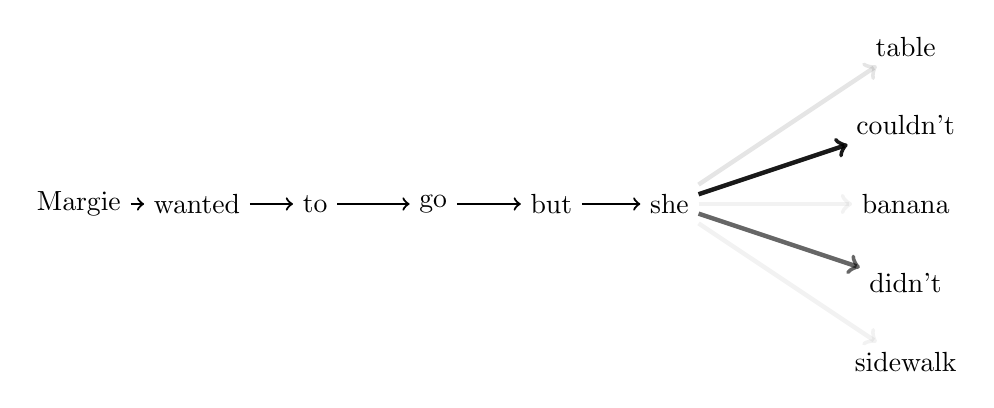
\begin{tikzpicture}[xscale = 1.5]
  \node (W1) at (0, 0) {
    Margie
  };


  \node (W2) at (1, 0) {
    wanted
  };

  \node (W3) at (2, 0) {
    to
  };

  \node (W4) at (3, 0) {
    go
  };

  \node (W5) at (4, 0) {
    but
  };

  \node (W6) at (5, 0) {
    she
  };

  \node (W7) at (7, 2) {
    table
  };

  \node (W8) at (7, 1) {
    couldn't
  };

  \node (W9) at (7, 0) {
    banana
  };

  \node (W10) at (7, -1) {
    didn't
  };

  \node (W11) at (7, -2) {
    sidewalk
  };

  \draw[thick, ->] (W1) -- (W2);
  \draw[thick, ->] (W2) -- (W3);
  \draw[thick, ->] (W3) -- (W4);
  \draw[thick, ->] (W4) -- (W5);
  \draw[thick, ->] (W5) -- (W6);
  \draw[ultra thick, ->, opacity = 0.1] (W6) -- (W7);
  \draw[ultra thick, ->, opacity = 0.9] (W6) -- (W8);
  \draw[ultra thick, ->, opacity = 0.05] (W6) -- (W9);
  \draw[ultra thick, ->, opacity = 0.6] (W6) -- (W10);
  \draw[ultra thick, ->, opacity = 0.05] (W6) -- (W11);
\end{tikzpicture}

    }
  \end{figure}

  \begin{itemize}
  \item Allows to learn the syntax of a language.
  \item Allows to learn the semantic of the words.
  \item Unlimited amount of data.
  \item Can be trained in multilingual setting.
  \end{itemize}

  \medskip

  The idea is to \textcolor{blue}{pretrain} a model using this task
  and then use what it has learned to perform some other tasks.
\end{frame}
%%%%%%%%%%%%%%%%%%%%%%%%%%%%%%%%%%%%%%%%%%%%%%%%%%%%%%%%%%%%%%%%%%%%%%

%%%%%%%%%%%%%%%%%%%%%%%%%%%%%%%%%%%%%%%%%%%%%%%%%%%%%%%%%%%%%%%%%%%%%%
\begin{frame}
  \frametitle{Google BERT}

  The \textbf{B}idirectional \textbf{E}ncoder \textbf{R}epresentations
  for \textbf{T}ransformers model is a language model that has been
  trained on a massive corpus (7000 books + all Wikipedia pages for
  102 languages). It is used as a \textcolor{blue}{base} to perform
  many other linguistic tasks.

  \bigskip

  It allows user to work easily in a \textcolor{blue}{wide variety of
    languages}.

  \bigskip

  It produces new state of the art results on \textcolor{blue}{11 NLP
    tasks}.

  \bigskip

  It is very fast and inexpensive to \textcolor{blue}{transfer} on a
  new task.

  \bigskip

  A multilingual BERT model trained on a \textcolor{blue}{monolingual
    dataset} will work (although with lower performances than with a
  proper training) on \textcolor{blue}{another language} (zero-shot
  learning).
\end{frame}
%%%%%%%%%%%%%%%%%%%%%%%%%%%%%%%%%%%%%%%%%%%%%%%%%%%%%%%%%%%%%%%%%%%%%%

%%%%%%%%%%%%%%%%%%%%%%%%%%%%%%%%%%%%%%%%%%%%%%%%%%%%%%%%%%%%%%%%%%%%%%
\begin{frame}
  \frametitle{References}

  \fontsize{6pt}{7.2}\selectfont

  \begin{itemize}
  \item IMDB movie review classification: \href{https://github.com/rodgzilla/pytorch-openai-transformer-lm/tree/movie_reviews_classification}{\textcolor{blue}{Github repo for IMDB sentiment analysis with GPT}}

  \item Convolution layer visualization: \href{https://www.matthewzeiler.com/research.html}{\textcolor{blue}{matthewzeiler.com}}

  \item Mikolov, Tomas, et al. "Distributed representations of words
    and phrases and their compositionality." Advances in neural
    information processing systems. 2013.

  \item Google blog post about gender bias in Google Translate:
    \href{https://www.blog.google/products/translate/reducing-gender-bias-google-translate/}{\textcolor{blue}{Reducing gender bias in Google Translate}} (2018)

  \item Chu, Eric, and Peter J. Liu. "Unsupervised Neural
    Multi-document Abstractive Summarization." arXiv preprint
    arXiv:1810.05739 (2018).

  \item Liu, Peter J., et al. "Generating wikipedia by summarizing
    long sequences." arXiv preprint arXiv:1801.10198 (2018).

  \item Devlin, Jacob, et al. "BERT: Pre-training of Deep
    Bidirectional Transformers for Language Understanding." arXiv
    preprint arXiv:1810.04805 (2018).

    \bigskip

  \item \href{https://github.com/rodgzilla/talk-slides/tree/master/machine_learning/general_focus_NLP}{\textcolor{blue}{Github repo for these slides.}}
  \end{itemize}
\end{frame}
%%%%%%%%%%%%%%%%%%%%%%%%%%%%%%%%%%%%%%%%%%%%%%%%%%%%%%%%%%%%%%%%%%%%%%

\appendix

%%%%%%%%%%%%%%%%%%%%%%%%%%%%%%%%%%%%%%%%%%%%%%%%%%%%%%%%%%%%%%%%%%%%%%
\begin{frame}
  \frametitle{Word2vec algorithm}

  The goal of the word2vec task is to predict the
  \textcolor{blue}{context} of word (the words surrounding it) based
  on its vector representation.

  \begin{center}
    \includegraphics[width = 4cm]{images/w2v.png}
  \end{center}
\end{frame}
%%%%%%%%%%%%%%%%%%%%%%%%%%%%%%%%%%%%%%%%%%%%%%%%%%%%%%%%%%%%%%%%%%%%%%

%%%%%%%%%%%%%%%%%%%%%%%%%%%%%%%%%%%%%%%%%%%%%%%%%%%%%%%%%%%%%%%%%%%%%%
\begin{frame}
  \frametitle{Unsupervised summarization model}

  The abstractive summary is generated by decoding the
  \textcolor{blue}{mean representation} of the input documents.

  \begin{center}
    \includegraphics[width = 12cm]{images/unsupervised_summarization_model.png}
  \end{center}
\end{frame}
%%%%%%%%%%%%%%%%%%%%%%%%%%%%%%%%%%%%%%%%%%%%%%%%%%%%%%%%%%%%%%%%%%%%%%

%%%%%%%%%%%%%%%%%%%%%%%%%%%%%%%%%%%%%%%%%%%%%%%%%%%%%%%%%%%%%%%%%%%%%%
\begin{frame}
  \frametitle{Google BERT for NLP tasks}

  To perform other tasks with BERT, you need to format your input and
  objective according to the way described in the article.

  \begin{center}
    \includegraphics[width = 7cm]{images/bert.png}
  \end{center}
\end{frame}
%%%%%%%%%%%%%%%%%%%%%%%%%%%%%%%%%%%%%%%%%%%%%%%%%%%%%%%%%%%%%%%%%%%%%%

\end{document}
